%%%%%%%%%%%%%%%%%%%%%%%%%%%%%%%%%%%%%%%%%
% Jacobs Landscape Poster
% LaTeX Template
% Version 1.1 (14/06/14)
%
% Created by:
% Computational Physics and Biophysics Group, Jacobs University
% https://teamwork.jacobs-university.de:8443/confluence/display/CoPandBiG/LaTeX+Poster
% 
% Further modified by:
% Nathaniel Johnston (nathaniel@njohnston.ca)
%
% This template has been downloaded from:
% http://www.LaTeXTemplates.com
%
% License:
% CC BY-NC-SA 3.0 (http://creativecommons.org/licenses/by-nc-sa/3.0/)
%
%%%%%%%%%%%%%%%%%%%%%%%%%%%%%%%%%%%%%%%%%

%----------------------------------------------------------------------------------------
%	PACKAGES AND OTHER DOCUMENT CONFIGURATIONS
%----------------------------------------------------------------------------------------

\documentclass[final]{beamer}
\usepackage[utf8]{inputenc}
\usepackage[scale=1.24]{beamerposter} % Use the beamerposter package for laying out the poster

\usetheme{confposter} % Use the confposter theme supplied with this template

\setbeamercolor{block title}{fg=ngreen,bg=white} % Colors of the block titles
\setbeamercolor{block body}{fg=black,bg=white} % Colors of the body of blocks
\setbeamercolor{block alerted title}{fg=white,bg=dblue!70} % Colors of the highlighted block titles
\setbeamercolor{block alerted body}{fg=black,bg=dblue!10} % Colors of the body of highlighted blocks
% Many more colors are available for use in beamerthemeconfposter.sty

%-----------------------------------------------------------
% Define the column widths and overall poster size
% To set effective sepwid, onecolwid and twocolwid values, first choose how many columns you want and how much separation you want between columns
% In this template, the separation width chosen is 0.024 of the paper width and a 4-column layout
% onecolwid should therefore be (1-(# of columns+1)*sepwid)/# of columns e.g. (1-(4+1)*0.024)/4 = 0.22
% Set twocolwid to be (2*onecolwid)+sepwid = 0.464
% Set threecolwid to be (3*onecolwid)+2*sepwid = 0.708

\newlength{\sepwid}
\newlength{\onecolwid}
\newlength{\twocolwid}
\newlength{\threecolwid}
\setlength{\paperwidth}{48in} % A0 width: 46.8in
\setlength{\paperheight}{36in} % A0 height: 33.1in
\setlength{\sepwid}{0.024\paperwidth} % Separation width (white space) between columns
\setlength{\onecolwid}{0.22\paperwidth} % Width of one column
\setlength{\twocolwid}{0.464\paperwidth} % Width of two columns
\setlength{\threecolwid}{0.708\paperwidth} % Width of three columns
\setlength{\topmargin}{-0.5in} % Reduce the top margin size
%-----------------------------------------------------------

\usepackage{graphicx}  % Required for including images

\usepackage{booktabs} % Top and bottom rules for tables

%----------------------------------------------------------------------------------------
%	TITLE SECTION 
%----------------------------------------------------------------------------------------

\title{Battlesnake using Deep Q Learning} % Poster title

\author{Petter Amundsen , Tommy Bergsvåg and Håkon Sagehaug  } % Author(s)

\institute{Bouvet} % Institution(s)

%----------------------------------------------------------------------------------------

\begin{document}

\addtobeamertemplate{block end}{}{\vspace*{2ex}} % White space under blocks
\addtobeamertemplate{block alerted end}{}{\vspace*{2ex}} % White space under highlighted (alert) blocks

\setlength{\belowcaptionskip}{2ex} % White space under figures
\setlength\belowdisplayshortskip{2ex} % White space under equations

\begin{frame}[t] % The whole poster is enclosed in one beamer frame

\begin{columns}[t] % The whole poster consists of three major columns, the second of which is split into two columns twice - the [t] option aligns each column's content to the top

\begin{column}{\sepwid}\end{column} % Empty spacer column

\begin{column}{\onecolwid} % The first column

%----------------------------------------------------------------------------------------
%	OBJECTIVES
%----------------------------------------------------------------------------------------

\begin{alertblock}{Objectives}
Make Deep Q learning neural network for training snakes used for playing the game \href{https://play.battlesnake.com/}{Battlesnake}
\begin{itemize}
\item Can we use Deep Q learning for training snakes to play the game
\item Can we make the AI snakes perform better than traditionally programmed snakes
\end{itemize}

\end{alertblock}

%----------------------------------------------------------------------------------------
%	INTRODUCTION
%----------------------------------------------------------------------------------------

\begin{block}{Introduction}

Poster for describing the work done for student project in INF626. We wanted to see if we could use Deep Q learning for training snakes for playing the game Battlesnake. Battlesnake is a game played on a squared board. For training we used an 11x11 board. The goal of the game is to survive. For a snake to survive it must; eat, not crash into other snakes and not crash into the wall - the last snake on the board is the winner. 

\end{block}

%------------------------------------------------

\begin{figure}
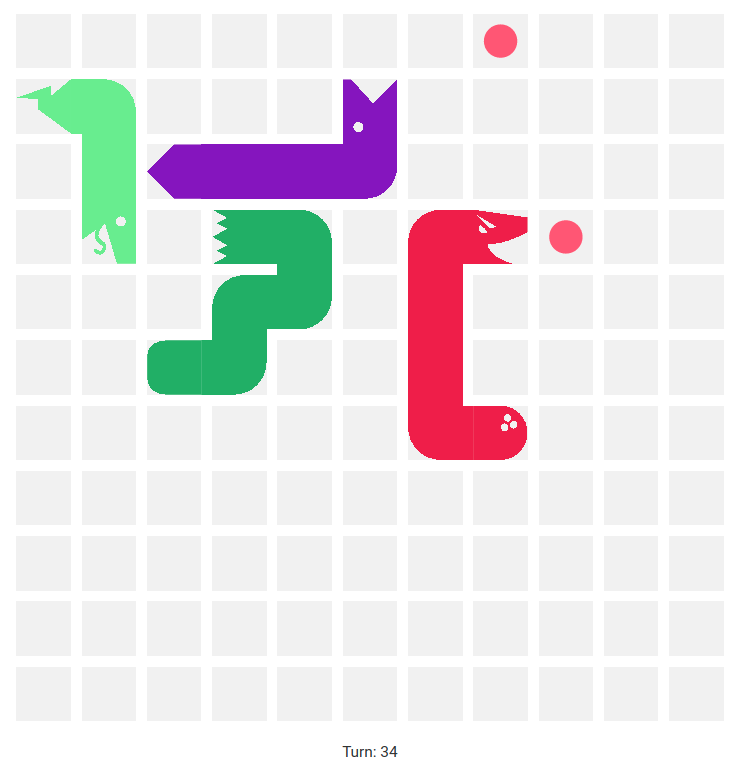
\includegraphics[width=1\linewidth]{battlesnake.png}
\caption{Battlesnakes game: 4 snakes compete in surviving the longest.	}
\end{figure}

%----------------------------------------------------------------------------------------

\end{column} % End of the first column

\begin{column}{\sepwid}\end{column} % Empty spacer column

\begin{column}{\twocolwid} % Begin a column which is two columns wide (column 2)

\begin{columns}[t,totalwidth=\twocolwid] % Split up the two columns wide column
			
\begin{column}{\onecolwid}\vspace{-.6in} % The first column within column 2 (column 2.1)

%----------------------------------------------------------------------------------------
%	METHOD
%----------------------------------------------------------------------------------------
\begin{figure}
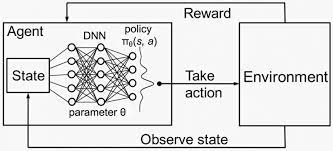
\includegraphics[width=1\linewidth]{deepq.jpeg}
\caption{Overview of deep Q network.}
\end{figure}

\begin{block}{Method}

Before each move the state of the game is fed to the agent as an 11x11 array, holding the coordinates of every snake head and body, as well as food. 
Before the network is properly trained it should do some exploration, trying random moves, so for every move there is a $\epsilon$ probability of the agent doing something at random. $\epsilon$ decays over time at an exponential rate, converging towards 0. 
For every action, there is a reward, and the neural network will adopt the weights that maximizes reward. The snakes have been given different reward functions for trying out different strategies. 
The neural network is implemented with Keras/Tensorflow. 
\end{block}

%----------------------------------------------------------------------------------------

\end{column} % End of column 2.1

\begin{column}{\onecolwid}\vspace{-.6in} % The second column within column 2 (column 2.2)

%----------------------------------------------------------------------------------------
%	METHODS
%----------------------------------------------------------------------------------------

\begin{block}{Implementation/Method}
			
Trained three different snakes each having a reward function

\begin{enumerate}
\item Snake only gets one point if is the only snake left meaning it won the game 					
\item Snake is punished when loosing the game, and rewarded when winning
\item Snake gets point if it survives
\end{enumerate}

Then we created three different models using Keras Sequential model with input
 \begin{enumerate}
\item Shape of the board(11x11) 					
\item Activation function, here we used ReLU and LeakeyReLU
\item One model with 2 layers and two with three layers
\end{enumerate}

\end{block}

%----------------------------------------------------------------------------------------

\end{column} % End of column 2.2

\end{columns} % End of the split of column 2 - any content after this will now take up 2 columns width

%----------------------------------------------------------------------------------------
%	IMPORTANT RESULT
%----------------------------------------------------------------------------------------

% \begin{alertblock}{Important Result}

% The snakes were able to play the game, but did not perform at a super-human level.

% \end{alertblock} 

%----------------------------------------------------------------------------------------

\begin{columns}[t,totalwidth=\twocolwid] % Split up the two columns wide column again

\begin{column}{\onecolwid} % The first column within column 2 (column 2.1)

%----------------------------------------------------------------------------------------
%	RESULTS
%----------------------------------------------------------------------------------------

\begin{block}{Results}

\begin{figure}
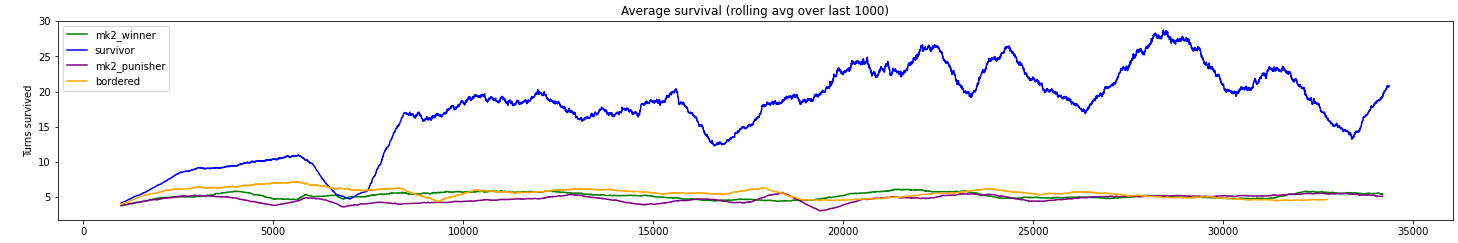
\includegraphics[width=0.8\linewidth]{average_survival.PNG}
\caption{Average survival measured in number of turns.}
\end{figure}


\begin{figure}
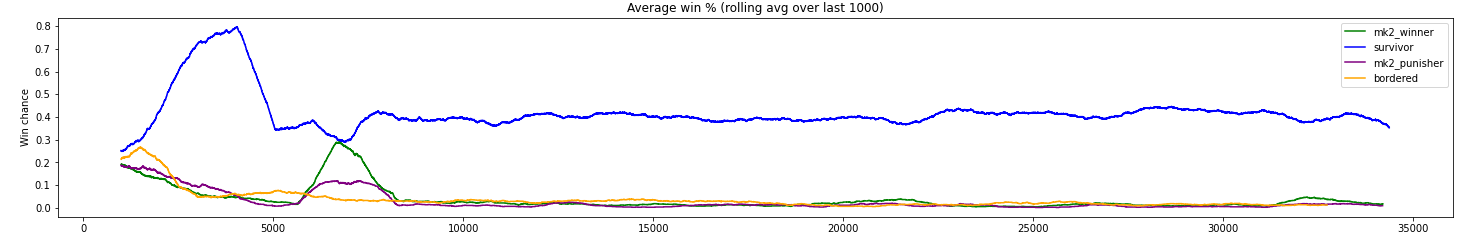
\includegraphics[width=0.8\linewidth]{win_chance.PNG}
\caption{Probability of winning for each snake, as the training progressed.}
\end{figure}

All the snakes performed better over time, but the snake named 'survivor' outperformed the others significantly. 
Additional training after the first 10000 games did not appear to increase performance. 
\end{block}
%----------------------------------------------------------------------------------------

\end{column} % End of column 2.1

\begin{column}{\onecolwid} % The second column within column 2 (column 2.2)
%----------------------------------------------------------------------------------------
%	DISCUSSION
%----------------------------------------------------------------------------------------

\begin{block}{Discussion}

Some bugs were discovered in the game code that prevented the snakes from learning. 
These issues were hard to troubleshoot and were discovered mostly by coincidence. 
There might be other such bugs lurking, preventing the snakes from performing at a superhuman level. 
It is also possible that the top snake is being held back by the other low performing snakes, as the game ends when there is just one snake left on the board. 
If we had replaced all the snakes with four identical 'survivor' snakes, we would likely have seen longer lasting games. 

\end{block}

%----------------------------------------------------------------------------------------

\end{column} % End of column 2.2

\end{columns} % End of the split of column 2

\end{column} % End of the second column

\begin{column}{\sepwid}\end{column} % Empty spacer column

\begin{column}{\onecolwid} % The third column

%----------------------------------------------------------------------------------------
%	CONCLUSION
%----------------------------------------------------------------------------------------

\begin{block}{Conclusion}

We set out to use reinforcement learning to train battlesnakes. 
The snakes did not perform at the expected level, but were much better than random chance. 

\end{block}

%----------------------------------------------------------------------------------------
%	ADDITIONAL INFORMATION
%----------------------------------------------------------------------------------------

\begin{block}{Additional Information}

Source code can be found on github: \href{https://github.com/petteramu/battlesnakes-dqn}{https://github.com/petteramu/battlesnakes-dqn}

\end{block}


%----------------------------------------------------------------------------------------
%	CONTACT INFORMATION
%----------------------------------------------------------------------------------------

\setbeamercolor{block alerted title}{fg=black,bg=norange} % Change the alert block title colors
\setbeamercolor{block alerted body}{fg=black,bg=white} % Change the alert block body colors

\begin{alertblock}{Contact Information}

\begin{itemize}
\item Petter Amundsen, petter.amundsen@bouvet.no
\item Håkon Sagehaug, hakon.sagehaug@bouvet.no
\item Tommy Bergsvåg, tommy.bergsvag@bouvet.no
\end{itemize}

\end{alertblock}

%----------------------------------------------------------------------------------------

\end{column} % End of the third column

\end{columns} % End of all the columns in the poster

\end{frame} % End of the enclosing frame

\end{document}
